% =============================================================================
% Ayndrome — Project Report (LaTeX)
% Compile: pdflatex Ayndrome_Project_Report.tex (run twice for TOC/refs)
%
% Note: Project_Report_Format.docx was not found at
%       C:/xampp2/htdocs/ayndrome_api (path does not exist on this machine).
%       Sections below follow a typical B.Tech / MCA project report outline.
%       Replace placeholders in \reportmeta{} with your institute details.
% =============================================================================

\documentclass[12pt,a4paper,oneside]{report}

\usepackage[margin=2.5cm]{geometry}
\usepackage[T1]{fontenc}
\usepackage[utf8]{inputenc}
\usepackage{lmodern}
\usepackage{microtype}
\usepackage{graphicx}
\usepackage{booktabs}
\usepackage{longtable}
\usepackage{array}
\usepackage{hyperref}
\usepackage{enumitem}
\usepackage{titlesec}
\usepackage{fancyhdr}
\usepackage{float}
\usepackage{caption}
\usepackage{subcaption}
\usepackage{tikz}
\usetikzlibrary{arrows.meta,positioning,shapes.geometric,fit,backgrounds,calc,shadows}
\usepackage{listings}
\usepackage{xcolor}
\usepackage{amsmath}

\hypersetup{
    colorlinks=true,
    linkcolor=blue!60!black,
    citecolor=green!50!black,
    urlcolor=blue!70!black
}

\lstdefinestyle{code}{
    basicstyle=\ttfamily\small,
    breaklines=true,
    frame=single,
    backgroundcolor=\color{gray!8},
    keywordstyle=\color{blue!70!black},
    commentstyle=\color{green!40!black},
    stringstyle=\color{orange!80!black},
    showstringspaces=false,
    tabsize=2
}
\lstset{style=code}

% --- Placeholders (edit before submission) ---
\newcommand{\projecttitle}{Ayndrome: Drone Delivery Platform}
\newcommand{\subtitle}{Full-Stack Web Application (React + Vite \& PHP API)}
\newcommand{\studentname}{[Student Name]}
\newcommand{\rollno}{[Roll Number]}
\newcommand{\guide}{[Guide Name]}
\newcommand{\institute}{[Institute / Department]}
\newcommand{\academicyear}{2025--2026}

\pagestyle{fancy}
\fancyhf{}
\fancyhead[L]{\small\leftmark}
\fancyhead[R]{\small Ayndrome Project Report}
\fancyfoot[C]{\thepage}
\renewcommand{\headrulewidth}{0.4pt}

% =============================================================================
\begin{document}

% -------------------- Title Page --------------------
\begin{titlepage}
    \centering
    \vspace*{1.5cm}
    {\Large \textbf{\institute}\par}
    \vspace{0.8cm}
    {\large DEPARTMENT OF [COMPUTER SCIENCE / IT]\par}
    \vspace{2cm}
    {\huge \textbf{\projecttitle}\par}
    \vspace{0.5cm}
    {\Large \subtitle\par}
    \vspace{2cm}
    {\large A Project Report\par}
    \vspace{0.3cm}
    {\large Submitted in partial fulfillment of the requirements\par}
    {\large for the degree of [B.Tech / MCA / BCA]\par}
    \vspace{2cm}
    \begin{tabular}{rl}
        \textbf{Submitted by:} & \studentname \\
        \textbf{Roll No.:}     & \rollno \\
        \textbf{Guide:}        & \guide \\
        \textbf{Academic Year:}& \academicyear \\
    \end{tabular}
    \vfill
    {\large \academicyear\par}
\end{titlepage}

\pagenumbering{roman}

% -------------------- Certificate (template) --------------------
\chapter*{Certificate}
\addcontentsline{toc}{chapter}{Certificate}
This is to certify that the project report entitled ``\projecttitle'' submitted by
\textbf{\studentname} (Roll No.~\rollno) is a bonafide record of work carried out under my
supervision at \institute{} during the academic year \academicyear.

\vspace{2cm}
\noindent
\begin{tabular}{@{}p{0.45\textwidth}@{\hfill}p{0.45\textwidth}@{}}
    \textbf{Guide} & \textbf{Head of Department} \\
    \guide & [HOD Name] \\
\end{tabular}

% -------------------- Declaration --------------------
\chapter*{Declaration}
\addcontentsline{toc}{chapter}{Declaration}
I hereby declare that this project report is my original work and has not been submitted
elsewhere for any degree or diploma. All sources have been acknowledged.

\vspace{1.5cm}
\noindent Place: \underline{\hspace{4cm}} \hfill Date: \underline{\hspace{3cm}}\\
\noindent Signature: \underline{\hspace{5cm}}\\
\noindent \studentname

% -------------------- Acknowledgement --------------------
\chapter*{Acknowledgement}
\addcontentsline{toc}{chapter}{Acknowledgement}
I express sincere gratitude to \guide{} and the faculty of \institute{} for guidance
throughout this project. Thanks are also due to peers and family for their support during
development and testing of the Ayndrome drone delivery platform.

% -------------------- Abstract --------------------
\chapter*{Abstract}
\addcontentsline{toc}{chapter}{Abstract}
Ayndrome is a full-stack drone parcel delivery platform comprising a \textbf{React 19 + Vite 6}
single-page application (\texttt{vite-project}) and a \textbf{flat PHP REST-style API}
(\texttt{api}) backed by \textbf{MySQL}. Users register, authenticate via email OTP, book
deliveries on interactive maps (Leaflet), pay for orders, and track drones in real time using
\textbf{Firebase Realtime Database}. Administrators monitor orders, block users, and respond to
issues through a dashboard with Chart.js analytics. Third-party integrations include
\textbf{PHPMailer}, \textbf{Twilio}, and \textbf{Kreait Firebase PHP}. The system targets local
deployment on \textbf{XAMPP} (Apache + MySQL) with the Vite dev server on port 5173.

\textbf{Keywords:} drone delivery, React, Vite, PHP, MySQL, Firebase, OTP authentication, SPA.

\tableofcontents
\listoffigures
\listoftables
\clearpage
\pagenumbering{arabic}

% =============================================================================
\chapter{Introduction}
% =============================================================================

\section{Background}
Last-mile logistics increasingly relies on automation. Ayndrome prototypes a consumer-facing
drone delivery service: marketing landing pages, authenticated booking flows, payment capture,
live tracking, and administrative oversight---implemented as a decoupled frontend and JSON API
suitable for academic demonstration and extension toward production hardening.

\section{Problem Statement}
Traditional courier interfaces rarely expose real-time aerial tracking or unified booking,
payment, and support in one experience. Ayndrome addresses:
\begin{itemize}[noitemsep]
    \item fragmented booking and tracking across separate tools;
    \item lack of live geospatial feedback during drone transit;
    \item limited admin visibility into orders, user issues, and account enforcement.
\end{itemize}

\section{Objectives}
\begin{enumerate}[label=\arabic*.]
    \item Design and implement a responsive web client for drone delivery booking.
    \item Build a PHP API with MySQL persistence and session-based security.
    \item Integrate Firebase for realtime drone position updates.
    \item Provide admin modules for analytics, notifications, and user moderation.
    \item Document architecture, data model, and deployment for reproducibility.
\end{enumerate}

\section{Scope and Limitations}
\textbf{In scope:} user auth (OTP), orders, rides, saved locations, payments (metadata),
tracking simulation, feedback, business contact, admin dashboard.

\textbf{Out of scope / limitations:}
\begin{itemize}[noitemsep]
    \item Physical drone hardware control (simulation workers update Firebase instead).
    \item Production payment gateway (card data stored as application metadata).
    \item Role-based admin enforcement (partially commented out in API).
    \item Centralized API router---each endpoint is a standalone PHP script.
\end{itemize}

% =============================================================================
\chapter{Literature Survey and Related Work}
% =============================================================================

Commercial platforms (e.g., food delivery, logistics SaaS) combine maps, payments, and
notifications. Ayndrome adopts similar patterns at smaller scale: SPA frontend, REST-like
backend, dual persistence (relational + realtime). Open-source stacks commonly pair
\textbf{React + Vite} for UI velocity and \textbf{PHP + MySQL} for shared hosting compatibility
(XAMPP), which informed technology choices for this academic deployment.

% =============================================================================
\chapter{System Analysis}
% =============================================================================

\section{Existing vs.\ Proposed System}
\begin{table}[H]
    \centering
    \caption{Comparison of manual process vs.\ Ayndrome}
    \label{tab:comparison}
    \begin{tabular}{@{}p{0.22\textwidth}p{0.36\textwidth}p{0.36\textwidth}@{}}
        \toprule
        \textbf{Aspect} & \textbf{Manual / Generic} & \textbf{Ayndrome} \\
        \midrule
        Booking & Phone / form, no map & Map-based pickup/dropoff \\
        Tracking & Static status codes & Firebase live coordinates \\
        Auth & Plain login & Password + email OTP session \\
        Admin & Spreadsheets & Dashboard + block user APIs \\
        \bottomrule
    \end{tabular}
\end{table}

\section{Functional Requirements}
\begin{itemize}
    \item \textbf{FR1:} User registration and login with OTP verification.
    \item \textbf{FR2:} Create and cancel delivery orders with scheduling and package details.
    \item \textbf{FR3:} Save payment methods and complete checkout flow.
    \item \textbf{FR4:} View delivery history, rides, saved locations, and submit feedback/issues.
    \item \textbf{FR5:} Real-time track active orders on map.
    \item \textbf{FR6:} Admin overview, user blocking, issue replies, notifications.
\end{itemize}

\section{Non-Functional Requirements}
\begin{itemize}
    \item \textbf{NFR1:} JSON API responses with CORS for Vite origin (\texttt{localhost:5173}).
    \item \textbf{NFR2:} Credential-bearing requests for PHP session cookies.
    \item \textbf{NFR3:} Error logging to \texttt{php\_errors.log} and \texttt{order\_creation.log}.
    \item \textbf{NFR4:} Responsive UI (Tailwind CDN, mobile-friendly components).
\end{itemize}

\section{Hardware and Software Requirements}
\begin{table}[H]
    \centering
    \caption{Development environment}
    \label{tab:env}
    \begin{tabular}{@{}ll@{}}
        \toprule
        \textbf{Category} & \textbf{Specification} \\
        \midrule
        OS & Windows 10/11 (project tested on Win 10.0.26200) \\
        Web server & Apache (XAMPP) \\
        Database & MySQL 8.x, database name \texttt{ayndrome} \\
        Frontend runtime & Node.js 18+, npm \\
        Backend runtime & PHP 8.x \\
        Browser & Chrome / Edge (latest) \\
        \bottomrule
    \end{tabular}
\end{table}

% =============================================================================
\chapter{System Design}
% =============================================================================

\section{Overall Architecture}
Figure~\ref{fig:architecture} shows the three-tier layout: browser SPA, PHP API on Apache, and
MySQL plus Firebase. Optional AI/voice services sit outside the core repo.

\begin{figure}[H]
    \centering
    \begin{tikzpicture}[
        node distance=1.1cm and 1.4cm,
        comp/.style={draw, rounded corners, align=center, minimum width=2.6cm,
                     minimum height=0.9cm, fill=blue!8, drop shadow},
        ext/.style={draw, dashed, rounded corners, align=center, minimum width=2.4cm,
                    fill=orange!10},
        arr/.style={-{Stealth[length=2.2mm]}, thick}
    ]
        \node[comp] (ui) {React SPA\\(Vite :5173)};
        \node[comp, right=of ui] (api) {PHP API\\(\texttt{/api/*.php})};
        \node[comp, below=of api] (db) {MySQL\\(\texttt{ayndrome})};
        \node[ext, above=of api] (fb) {Firebase RTDB\\(\texttt{drones\_tracking})};
        \node[ext, left=1.8cm of ui] (mail) {PHPMailer\\OTP / alerts};
        \node[ext, right=1.8cm of api] (twilio) {Twilio\\voice/SMS};
        \node[ext, below=of ui] (ai) {Voice AI\\(localhost:5000)};

        \draw[arr] (ui) -- node[above, font=\small]{fetch + cookies} (api);
        \draw[arr] (api) -- (db);
        \draw[arr] (api) -- (fb);
        \draw[arr] (ui) -- node[left, font=\small]{SDK subscribe} (fb);
        \draw[arr] (api) -.-> (mail);
        \draw[arr] (api) -.-> (twilio);
        \draw[arr] (ui) -.-> (ai);
    \end{tikzpicture}
    \caption{High-level system architecture}
    \label{fig:architecture}
\end{figure}

\section{Module Decomposition}
\subsection{Frontend (\texttt{vite-project})}
\begin{itemize}
    \item \textbf{Landing} (\texttt{appleclone.jsx}): marketing, Three.js drone hero, voice hook.
    \item \textbf{App shell} (\texttt{droneapp.jsx}): auth gate, nested routes, navbar/footer.
    \item \textbf{Booking flow}: \texttt{landingPage}, \texttt{Map}, \texttt{DeliveryDetails},
          \texttt{Payment}, \texttt{OrderConfirmation}, \texttt{Tracking}.
    \item \textbf{Account}: \texttt{login}, \texttt{signUp}, \texttt{OTPVerification}, \texttt{Profile}.
    \item \textbf{Admin}: \texttt{AdminDashboard} and sub-panels (overview, block user, issues).
\end{itemize}

\subsection{Backend (\texttt{api})}
Approximately \textbf{65 PHP endpoint scripts}, each exposing JSON over HTTP. Shared includes:
\texttt{cors.php}, \texttt{db\_connect.php}, \texttt{utils.php}, \texttt{session.php},
\texttt{firebase\_helper.php}.

\subsection{Supporting (\texttt{ai})}
Dialogflow-style webhook stubs (\texttt{dialogflow\_webhook.php}, \texttt{intent\_handler.php})
for future voice intent routing.

\section{Database Design}
Core entities: \texttt{users}, \texttt{users\_orders}, \texttt{rides}, \texttt{saved\_locations},
\texttt{delivery\_history}, \texttt{track\_parcels}, \texttt{users\_activity},
\texttt{saved\_payment}, \texttt{delivery\_feedback}, \texttt{business\_contacts}.

\begin{figure}[H]
    \centering
    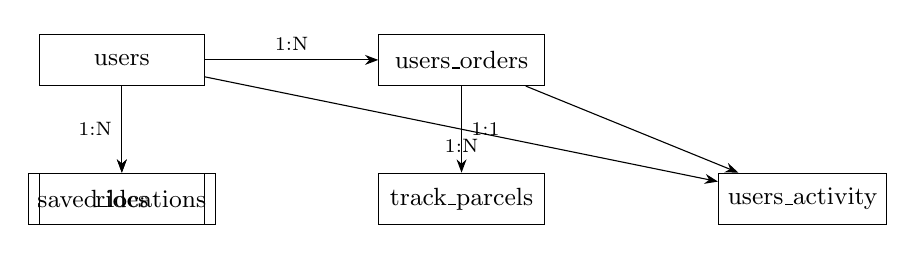
\begin{tikzpicture}[
        ent/.style={draw, rectangle, minimum width=2.1cm, minimum height=0.65cm,
                    align=center, font=\small},
        rel/.style={font=\scriptsize}
    ]
        \node[ent] (u) {users};
        \node[ent, right=2.2cm of u] (o) {users\_orders};
        \node[ent, below=1.1cm of o] (t) {track\_parcels};
        \node[ent, left=2.2cm of t] (r) {rides};
        \node[ent, below=1.1cm of u] (sl) {saved\_locations};
        \node[ent, right=2.2cm of t] (ua) {users\_activity};

        \draw[-{Stealth}] (u) -- node[rel, above]{1:N} (o);
        \draw[-{Stealth}] (o) -- node[rel, right]{1:1} (t);
        \draw[-{Stealth}] (u) -- node[rel, left]{1:N} (r);
        \draw[-{Stealth}] (u) -- (sl);
        \draw[-{Stealth}] (u) -- node[rel, below]{1:N} (ua);
        \draw[-{Stealth}] (o) -- (ua);
    \end{tikzpicture}
    \caption{Simplified entity-relationship diagram (core tables)}
    \label{fig:er}
\end{figure}

\section{Authentication Flow}
\begin{figure}[H]
    \centering
    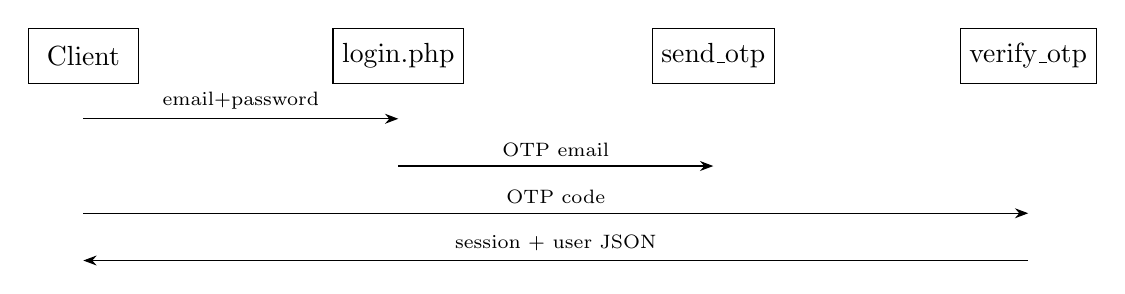
\begin{tikzpicture}[
        actor/.style={rectangle, draw, minimum height=0.7cm, minimum width=1.4cm, align=center},
        msg/.style={-{Stealth}, font=\scriptsize}
    ]
        \node[actor] (c) at (0,0) {Client};
        \node[actor] (l) at (4,0) {login.php};
        \node[actor] (o) at (8,0) {send\_otp};
        \node[actor] (v) at (12,0) {verify\_otp};

        \draw[msg] (0,-0.8) -- node[above]{email+password} (4,-0.8);
        \draw[msg] (4,-1.4) -- node[above]{OTP email} (8,-1.4);
        \draw[msg] (0,-2.0) -- node[above]{OTP code} (12,-2.0);
        \draw[msg] (12,-2.6) -- node[above]{session + user JSON} (0,-2.6);
    \end{tikzpicture}
    \caption{Login and OTP verification sequence}
    \label{fig:auth-seq}
\end{figure}

Sessions store \texttt{\$_SESSION['user\_id']} etc.; the client mirrors user data in
\texttt{localStorage} after successful OTP verification.

\section{Order and Tracking Flow}
\begin{figure}[H]
    \centering
    \begin{tikzpicture}[
        step/.style={draw, trapezium, trapezium left angle=70, trapezium right angle=110,
                     align=center, minimum width=2.2cm, fill=green!10},
        arr/.style={-{Stealth}, thick}
    ]
        \node[step] (a) {Map / booking};
        \node[step, right=1.2cm of a] (b) {create\_order.php};
        \node[step, right=1.2cm of b] (c) {MySQL row};
        \node[step, right=1.2cm of c] (d) {simulate\_drone};
        \node[step, right=1.2cm of d] (e) {Firebase update};
        \node[step, below=1.3cm of c] (f) {Tracking.jsx};

        \foreach \x/\y in {a/b, b/c, c/d, d/e}
            \draw[arr] (\x) -- (\y);
        \draw[arr] (e) -- (f);
        \draw[arr] (c) -- (f);
    \end{tikzpicture}
    \caption{Order creation and realtime tracking pipeline}
    \label{fig:order-flow}
\end{figure}

\section{Frontend Routing}
Top-level routes (\texttt{src/main.jsx}):
\begin{center}
    \texttt{/} $\rightarrow$ landing \quad
    \texttt{/app/*} $\rightarrow$ drone app \quad
    \texttt{/admin} $\rightarrow$ admin dashboard
\end{center}

Nested \texttt{/app/*} routes (\texttt{droneapp.jsx}) include
\texttt{map}, \texttt{delivery-details}, \texttt{payment}, \texttt{profile}, \texttt{track},
\texttt{login}, \texttt{signup}, \texttt{admin}, etc. Protected routes:
\texttt{delivery-details}, \texttt{payment}, \texttt{profile}, \texttt{order-confirmation}.

% =============================================================================
\chapter{Implementation}
% =============================================================================

\section{Technology Stack}
\begin{table}[H]
    \centering
    \caption{Technology summary}
    \label{tab:stack}
    \begin{tabular}{@{}lll@{}}
        \toprule
        \textbf{Layer} & \textbf{Technology} & \textbf{Version (from manifest)} \\
        \midrule
        UI framework & React & 19.x \\
        Build tool & Vite & 6.2 \\
        Routing & react-router-dom & 7.4 \\
        Maps & Leaflet + plugins & 1.9 / 3.x \\
        Charts & Chart.js, react-chartjs-2 & 4.4 / 5.3 \\
        Realtime client & Firebase JS & 11.6 \\
        API & PHP (flat scripts) & 8.x (server-dependent) \\
        ORM & None (raw PDO / mysqli) & --- \\
        Mail / SMS / Firebase admin & PHPMailer, Twilio, Kreait & composer.json \\
        \bottomrule
    \end{tabular}
\end{table}

\section{Project Directory Structure}
\begin{lstlisting}[language=bash, caption={Repository layout (abbreviated)}]
ayndrome-api/
  api/                 # PHP JSON endpoints, SQL migrations, logs
  vite-project/        # React + Vite frontend
    src/main.jsx       # Application entry and top routes
    public/components/ # Primary UI modules (unusual but intentional)
  ai/                  # Dialogflow / voice stubs
  composer.json        # PHP dependencies
\end{lstlisting}

\section{API Integration Pattern}
The frontend calls a fixed base URL:
\begin{lstlisting}[language=JavaScript]
const API = 'http://localhost/ayndrome-api/api/';
fetch(API + 'check_session.php', { credentials: 'include' });
\end{lstlisting}
\texttt{cors.php} reflects the request origin and enables credentials; sessions start on
included scripts. Example endpoints:

\begin{longtable}{@{}p{0.32\textwidth}p{0.14\textwidth}p{0.48\textwidth}@{}}
    \toprule
    \textbf{Endpoint} & \textbf{Method} & \textbf{Purpose} \\
    \midrule
    \endhead
    signup.php & POST & Register user, hashed password \\
    login.php & POST & Validate credentials, trigger OTP \\
    verify\_otp.php & POST & Validate OTP, create session \\
    check\_session.php & GET & Session probe for SPA \\
    create\_order.php & POST & Persist order (auth required) \\
    cancel\_order.php & POST & Cancel active order \\
    simulate\_drone\_delivery.php & --- & Drive tracking simulation \\
    admin\_dashboard\_overview.php & GET & Admin metrics \\
    admin\_block\_user.php & POST & Block/unblock accounts \\
    delivery\_feedback.php & GET/POST & Ratings and comments \\
    \bottomrule
\end{longtable}

\section{Database Connection}
\texttt{db\_connect.php} opens PDO and mysqli to \texttt{localhost}, database
\texttt{ayndrome}, user \texttt{root} (empty password in development). Production deployments
must use secrets management and least-privilege DB users.

\section{Firebase Integration}
Server-side \texttt{firebase\_helper.php} uses Kreait to \texttt{set()} paths such as
\texttt{drones\_tracking/\{order\_id\}}. Client \texttt{public/firebase.js} subscribes for live
UI updates in \texttt{Tracking.jsx} and profile views.

\section{Notable Implementation Details}
\begin{itemize}
    \item Dual DB APIs (PDO + mysqli) coexist across scripts---consolidation would reduce bugs.
    \item UI components live under \texttt{public/components/} while shadcn-style primitives sit
          in \texttt{src/components/ui/}.
    \item \texttt{App.jsx} is unused; \texttt{main.jsx} is the true entry point.
    \item Admin authorization checks are disabled in some scripts (security debt).
\end{itemize}

% =============================================================================
\chapter{Testing}
% =============================================================================

\section{Test Strategy}
\begin{itemize}
    \item \textbf{Unit-level:} manual verification of individual PHP endpoints via Postman or
          \texttt{ApiTest.jsx}.
    \item \textbf{Integration:} end-to-end booking from map $\rightarrow$ payment $\rightarrow$
          tracking with session cookies enabled.
    \item \textbf{UI:} responsive checks on mobile widths; map tile loading; toast notifications.
\end{itemize}

\section{Sample Test Cases}
\begin{table}[H]
    \centering
    \caption{Representative test cases}
    \label{tab:tests}
    \begin{tabular}{@{}clcc@{}}
        \toprule
        \textbf{ID} & \textbf{Description} & \textbf{Expected} & \textbf{Status} \\
        \midrule
        T1 & Valid signup & 201/200 JSON success & Manual \\
        T2 & Login + OTP & Session cookie set & Manual \\
        T3 & Protected route w/o auth & Redirect to login & Pass (client) \\
        T4 & Create order & Row in \texttt{users\_orders} & Manual \\
        T5 & Firebase tracking update & Map marker moves & Manual \\
        T6 & Admin block user & \texttt{blocked=1} in DB & Manual \\
        \bottomrule
    \end{tabular}
\end{table}

\section{Deployment Diagram}
\begin{figure}[H]
    \centering
    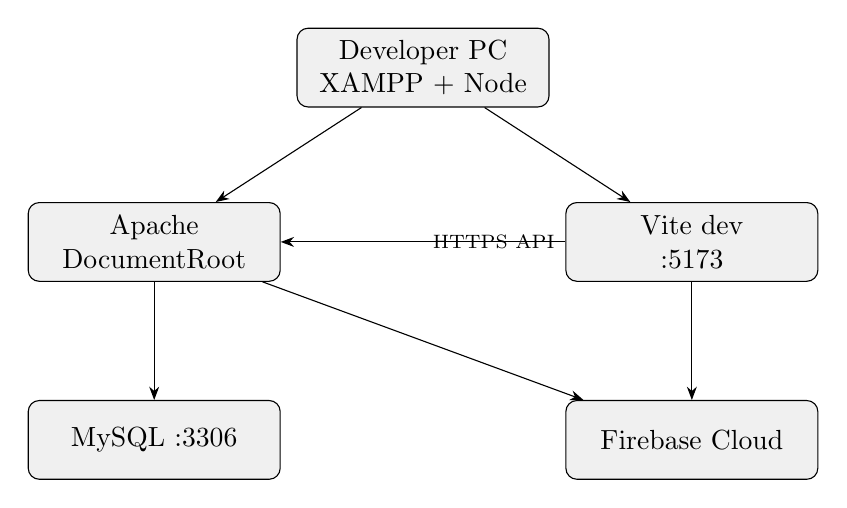
\begin{tikzpicture}[
        box/.style={draw, rounded corners, minimum width=3.2cm, minimum height=1cm,
                    align=center, fill=gray!12}
    ]
        \node[box] (dev) {Developer PC\\XAMPP + Node};
        \node[box, below left=1.2cm and 0.2cm of dev] (apache) {Apache\\DocumentRoot};
        \node[box, below right=1.2cm and 0.2cm of dev] (vite) {Vite dev\\:5173};
        \node[box, below=1.5cm of apache] (mysql) {MySQL :3306};
        \node[box, below=1.5cm of vite] (cloud) {Firebase Cloud};

        \draw[-{Stealth}] (dev) -- (apache);
        \draw[-{Stealth}] (dev) -- (vite);
        \draw[-{Stealth}] (apache) -- (mysql);
        \draw[-{Stealth}] (vite) -- node[right, font=\scriptsize]{HTTPS API} (apache);
        \draw[-{Stealth}] (vite) -- (cloud);
        \draw[-{Stealth}] (apache) -- (cloud);
    \end{tikzpicture}
    \caption{Local deployment topology (development)}
    \label{fig:deploy}
\end{figure}

\section{Installation Steps}
\begin{enumerate}
    \item Import SQL scripts from \texttt{api/create\_tables.sql} and related migrations into
          MySQL; create database \texttt{ayndrome}.
    \item Run \texttt{composer install} at repository root; configure PHPMailer and Twilio env.
    \item Place project under \verb|C:\xampp2\htdocs\ayndrome-api|.
    \item In \texttt{vite-project}: \texttt{npm install \&\& npm run dev}.
    \item Open \texttt{http://localhost:5173} and ensure API base URL matches Apache alias.
\end{enumerate}

% =============================================================================
\chapter{Results and Discussion}
% =============================================================================

The integrated system demonstrates a complete drone-delivery \emph{prototype}: users complete
authenticated bookings, operators can simulate drone movement into Firebase, and administrators
review traffic and support tickets. Performance is adequate for localhost demos; production
would require HTTPS, hardened secrets, payment PCI compliance, and API gateway patterns.

\textbf{Strengths:} clear separation of SPA and API; rich feature surface (profile, admin,
feedback); realtime tracking UX.

\textbf{Weaknesses:} flat PHP surface area (65 files), inconsistent fetch base paths, exposed
service account path in repo, disabled admin RBAC, and development DB credentials in source.

% =============================================================================
\chapter{Conclusion and Future Work}
% =============================================================================

Ayndrome successfully combines a modern React client with a PHP/MySQL backend and Firebase
realtime layer to model drone parcel delivery. Future work includes JWT or OAuth2, unified API
routing (Slim/Laravel), payment gateway integration, automated tests (PHPUnit, Vitest), CI/CD,
and hardware telemetry ingestion from actual UAV flight controllers.

% =============================================================================
\chapter*{References}
\addcontentsline{toc}{chapter}{References}
\begin{enumerate}[label={[\arabic*]}]
    \item React Documentation, \url{https://react.dev/}
    \item Vite Guide, \url{https://vite.dev/}
    \item PHP Manual, \url{https://www.php.net/manual/en/}
    \item Firebase Realtime Database, \url{https://firebase.google.com/docs/database}
    \item Leaflet, \url{https://leafletjs.com/}
    \item Kreait Firebase PHP, \url{https://firebase-php.readthedocs.io/}
\end{enumerate}

\appendix
\chapter{API Endpoint Inventory (Grouped)}
\begin{longtable}{@{}p{0.38\textwidth}p{0.58\textwidth}@{}}
    \toprule
    \textbf{Group} & \textbf{Files} \\
    \midrule
    \endhead
    Authentication &
    signup, login, verify\_otp, logout, check\_session, forgot\_password, reset\_password,
    change\_password, send\_otp \\
    Orders \& tracking &
    create\_order, cancel\_order, update\_order\_status, get\_track\_parcels, sync\_track\_parcels,
    simulate\_drone\_delivery, simulate\_drone\_worker, polling\_worker \\
    User profile &
    get\_user, get\_user\_profile, update\_profile, delete\_account, get\_rides, save\_ride,
    locations, saved\_locations \\
    Payments &
    save\_card, get\_saved\_cards \\
    Admin &
    admin\_dashboard\_overview, admin\_block\_user, get\_all\_users, admin\_user\_orders,
    admin\_user\_issues, admin\_reply\_issue, admin\_orders\_traffic, get/send\_admin\_notification \\
    Utilities &
    cors, db\_connect, firebase\_helper, reverse\_geocode, check\_blocked, business\_contact \\
    \bottomrule
\end{longtable}

\chapter{Report Format Note}
\textbf{Project\_Report\_Format.docx} was requested at
\texttt{C:/xampp2/htdocs/ayndrome\_api} but that directory and file were not present on the
analyzed machine (workspace path: \texttt{ayndrome-api} with hyphen). If your institute template
uses different chapter titles (e.g., ``Chapter 3: Methodology''), rename sections in this
\LaTeX{} source accordingly and recompile.

\end{document}
